\documentclass{article}
\usepackage[utf8]{inputenc}
\usepackage{csquotes}
\usepackage{todonotes}
\usepackage{amsmath}
\usepackage{graphicx}
\usepackage{relsize}
\usepackage{subcaption}

\title{Quick and Efficient Cross-chain Asset Exchange using Multi-signature Transactions and Witnesses}
\author{Martijn de Vos}
\date{April 2021}

\begin{document}

\maketitle

\section{Introduction}
TODO introduce topic

A common approach to exchange assets residing on different blockchains is by using \emph{atomic swaps}~\cite{herlihy2018atomic}.
An atomic swap is a coordination task where assets are either exchanged between parties or nothing happens.
This makes it a relatively secure mechanism to trade values across isolated blockchain environments.
The \enquote{traditional} atomic swap between two parties, Alice and Bob, uses hash-lock and time-lock transaction primitives to refund assets to one of the trading parties when the counterparty becomes inactive.

While atomic swaps seem to be the standard approach for cross-chain asset exchange without trusted intermediary (and also are foundational for many layer-two solutions~\cite{gudgeon2019sok}), this approach has deficiencies for the involved parties.
First, not all blockchain have native support for atomic swaps, and some protocols do not support hash- or time-locks.
Second, recent work shows that atomic swaps are susceptible for collusion with the operators of the involved blockchains~\cite{tsabary2020mad}.
In particular, a malicious user can bribe a miner to ignore the claim transaction of the counterparty, effectively confiscating their funds.
Third, atomic swaps are proven to be unfair for one of the parties since it effectively provides the counterparty with a free option and freely speculate on the price of an asset being traded~\cite{han2019optionality}.

In this work, we describe an alternative approach for quick and efficient exchange of value between different blockchains.
Our approach orients around multi-signature transactions and requires witnesses to digitally sign transactions associated with a particular trade to enforce its atomicity.
A key advantage is that the majority of the computations required by our system do not involve expensive on-chain transactions but are instead off-chain, performed by users themselves.
This significantly increases efficiency and throughput of our approach, requiring minimal interaction with the blockchains.
By leveraging a lightweight accountability mechanism, we enable any participant to detect and prove the wrongdoings of a trader or witness, resulting in quick community exclusion.\todo{finish + add numbers}

\section{Problem Description}
This work focusses on the problem of two users wanting to securely exchange assets between different blockchain platforms.
Assume, for example, that Alice wants to buy Bitcoin for Ethereum while Bob wants to sell his Ethereum for Bitcoin.
Furthermore, assume that Alice and Bob have no prior trust relation (e.g., they do not know each others real-world identity).
Then, these two users reach an agreement to trade (e.g., containing the pricing information of the assets to be traded) and the process of exchanging assets, or \emph{settlement} can start.
A naive approach is to have both Alice and Bob issue a Bitcoin and Ethereum transaction respectively where they transfer the agreed amounts of assets to the counterparty.
We refer to the transaction issued by Alice as $ tx_a $ and the transaction of Bob as $ tx_b $.
This unsupervised process, however, is risky: Alice or Bob can refrain from issuing the transaction, possibly resulting in a net loss for one of the parties.
The objective of an atomic swap is to prevent this exact situations: one transaction cannot complete without the other going through.

To address the lack of trust between traders, it is common to use a trusted intermediary, e.g., a cryptocurrency exchange, to process the trade.
The popularity of blockchain technology and different decentralized applications has resulted in the deployment of many cryptocurrency exchanges, some of them processing millions worth of transactions daily.
This approach requires Alice and Bob to trust that the intermediary correctly completes the trade and does not default or comprise the incoming assets.\todo{finish}
For an overview of state-of-the-art cross-chain trading mechanisms, we refer to reader to our prior work~\cite{de2021xchange}.\todo{list trust assumptions for each trading mechanism?}

As such, the overarching research question of this work is as follows: \emph{how can two users securely exchange assets between isolated blockchain platforms without involvement of a trusted intermediary?}

\begin{figure}[t]
	\centering
	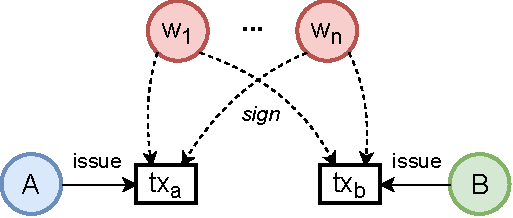
\includegraphics[width=.7\linewidth]{assets/trade_with_witnesses}
	\caption{A trade between Alice ($a$) and Bob ($ b $), assisted by $ n $ witnesses ($ w_1 \dots w_n) $. The issued transactions by Alice and Bob ($ tx_a $ and $ tx_b $, respectively) are signed by the involved witnesses.}
	\label{fig:trade_with_witnesses}
\end{figure}

\section{System and Threat Model}

\subsection{System Model}
We assume well-established membership.
This means that the digital identity of each peer in the network is tied to a real-world identity, e.g., through a certification by a trusted party.
This assumptions is required to address the Sybil Attack, the situation where an adversary subverts the network by creating many identities or by rejoining the network under a different identity~\cite{douceur2002sybil}.

\subsection{Threat Model}
TODO\todo{write}

\section{Efficient Asset Exchange using Witnesses}
We present an efficient approach to enable cross-chain asset exchange by leveraging multi-signature transactions and signature thresholds.
For presentation clarity, we first focus on permissioned networks where the identity of every user is well-established.
Our main idea is to have one or more witnesses that co-sign the transactions issued by two users that are exchanging assets.
This idea is visualized in Figure~\ref{fig:trade_with_witnesses}, showing a trade between Alice and Bob.
Both Alice and Bob issue a transaction that transfers assets to the counterparty (denoted as $ tx_a $ and $ tx_b $, respectively), but each transaction also has to be signed by one or more witnesses for inclusion in the blockchain.
We refer to the set of all witnesses in the network as $ W $, and the witnesses required to co-sign a transaction in trade $ T $ as $ W_T $.
The function $ V(\cdot) $ takes a transaction as input and outputs 1 if the transaction has enough signatures for its execution, and 0 otherwise.
This approach resembles a trade coordinated by a trusted escrow where the signature of the escrow is decisive to complete the trade.
However, we aim to avoid the need for a trusted party when trading.
Instead, we ask random users in the network to act as witness, therefore sidestepping the need for a singular trusted escrow.

The approach as depicted in Figure~\ref{fig:trade_with_witnesses} prevents Alice or Bob from \enquote{stealing} assets from the other party.
In addition, witnesses are not able to compromise assets since they are not in possession of the funds being transferred at any point during the trade as would be the case with escrow-based asset trade.
A dispute would arise if either $ tx_a $ goes through and $ tx_b $ does not go through, or vice versa.
Achieving this would require \emph{collusion} with witnesses where one trading party secretly collaborates with a subset of witnesses to compromise assets.
This collusion would work as follows: assume that Alice colludes with the witnesses that are co-signing the transactions of one of her trades.
She can now compromise Bobs' assets by having the witnesses refrain from signing $ tx_a $ while having the witnesses sign $ tx_b $.
As such, Bobs' assets would be transferred to Alice while Alice effectively retains control over her funds since $ tx_a $ will not be executed.

At this point, we have to answer the following two questions:
\begin{enumerate}
	\item How is the set of witnesses ($ W_T $) determined for each trade $ T $?
	\item How many signatures are required for a transaction to be satisfied?
\end{enumerate}

\subsection{Selecting Witnesses}
TODO\todo{write}

\begin{figure*}[t]
       \centering
       \begin{subfigure}[t]{.5\textwidth}
               \centering
               \captionsetup{width=.9\linewidth}
               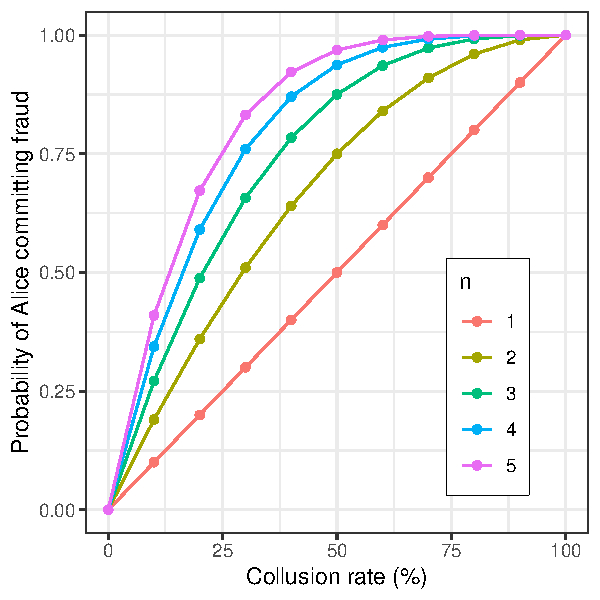
\includegraphics[width=.9\linewidth]{assets/fraud_probability_n_out_of_n.pdf}
               \caption{Using $n$-out-of-$n$ signatures.}
               \label{fig:prob_fraud_n_out_of_n_signatures}
       \end{subfigure}%
       \begin{subfigure}[t]{.5\textwidth}
               \centering
               \captionsetup{width=.9\linewidth}
               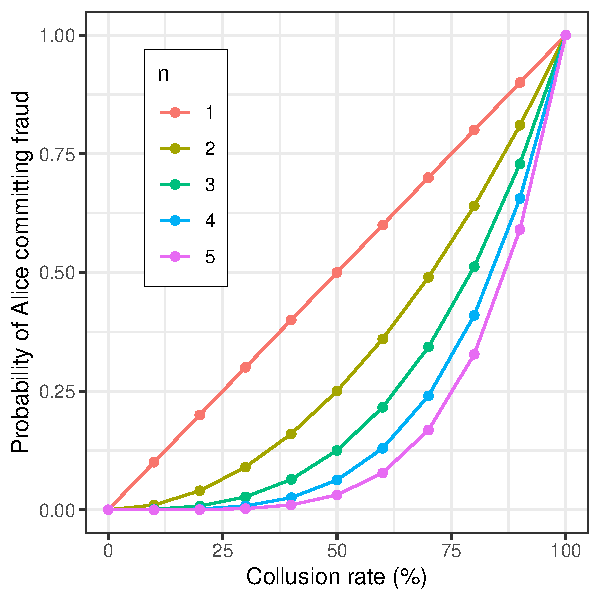
\includegraphics[width=.9\linewidth]{assets/fraud_probability_1_out_of_n.pdf}
               \caption{Using $1$-out-of-$n$ signatures.}
               \label{fig:prob_fraud_1_out_of_n_signatures}
       \end{subfigure}%
       \caption{The probabilities of Alice successfully committing fraud, for n-out-of-n and 1-out-of-n threshold signatures.}
       \label{fig:prob_fraud_signatures}
\end{figure*}

\subsection{Signature Thresholds}
The second question to answer is how many signatures are required for a particular transaction to be included on the involved blockchain.

\textbf{$n$-out-of-$n$ threshold.}
First, we analyse the situation where the signatures of all witnesses are required for a transaction to be executed.
Assume a trade between Alice and Bob using four witnesses ($ n = 4 $), and that Alice is colluding with one or more witnesses whereas Bob is honest.
Now, if Alice colludes with a single witness, she can direct the witness to refrain from signing $ tx_a $ while signing $ tx_b $, effectively leaving Bob with an economic loss.
As such, $n$-out-of-$n$ signatures are particularly vulnerable for collusion.
Specifically, if we assume random witness selection, and that Alice is colluding with fraction $ f $ of all witnesses in the network, the probability that $ tx_a $ will not be executed while $ tx_b $ can be modelled as follows:

\begin{equation}
	\begin{aligned}
	P(V(tx_a) = 0 \cap V(tx_b) = 1) & = P(V(tx_a) = 0)\\
	& = 1 - P(V(tx_a) = 1)\\
	& = 1 - (1 - f)^n
	\end{aligned}
\end{equation}

Note that we have assumed that Bob is honest and thus does not collude with any witness.
Therefore, $ P(V(tx_b) = 1) = 1 $ since both honest witnesses and witnesses colluding with Alice will sign for $ tx_b $.
If Alice colludes with 50\% of all witnesses, and each trade requires 5 witnesses, her fraud has a likelihood of ~96.9\% to succeed.
Specifically, Alice only requires collusion with only a single witness for her attack to succeed.
We have also plotted these probabilities in Figure~\ref{fig:prob_fraud_n_out_of_n_signatures}.
This figures shows that the probability of Alice committing fraud quickly increases for larger values of $ n $ and $ f $.
It also shows that it is preferred to utilize a low number of witnesses.

\textbf{$1$-out-of-$n$ threshold.}
If instead we assume an $1$-out-of-$n$ threshold scheme, it is required that Alice colludes with all witnesses of a trade.
The probability of her succeeding with $ n $ witnesses is modelled as followed:

\begin{equation}
	P(V(tx_a) = 0) = f^n
\end{equation}

The probability of Alice succeeding her fraud quickly decreases: even when Alice colludes with 50\% of all witnesses, requiring 5 witnesses for each trade already reduces her chance of succeeding to ~3.1\%.
We have visualized these probabilities in Figure~\ref{fig:prob_fraud_n_out_of_n_signatures}.
As opposed to the probabilities under the $n$-out-of-$n$ threshold scheme, we now see that we can keep the probability of Alice successfully committing fraud lower when we include more witnesses in our transactions.

While this scheme at a first glance might seem robust, the above scheme assumes that both traders actually generate and issue their transaction.
Without this assumption, there is a race condition here that would easily result in Alice committing fraud.
In particular, if Bob issues his transaction $tx_b$ (without any witness signatures) in the network first, and Alice colludes with a single witness, that single witness can sign $ tx_b $ and submit it to the blockchain network for execution.
Now, Alice refrains from sending out her transaction $tx_a$.
In this scenario, she has successfully compromised Bobs' assets.

\textbf{$t$-out-of-$n$ threshold.}
We now consider the scenario where we require a fraction of witnesses for a transaction to be executed.
We refer as the number of (valid) signatures required for transaction execution as $ t $ (where $ t \leq n $).
We can model the decision of each witness to sign a particular transaction as a Bernoulli trial.
Using a $t$-out-of-$n$ threshold scheme, this directly results in the following formula that gives the probability of Alice her attack succeeding:

\begin{equation}
	P(V(tx_a) = 0) = \mathlarger{\sum}_{i=t}^n {n \choose i} (1-f)^i f^{n-i}
\end{equation}

% Idea: witnesses should not sign without having seen both transactions
% We can devise an accountable MPC multi-sig computation.
% Weaken the assumption of full network knowledge by having both parties propose a few witnesses. Parties try their best to check if these witnesses are 'secure' enough.

\section{Making Witnesses Liable with Accountability}
TODO

\section{Related Work}
Bisq is a non-custodial and peer-to-peer trading network that uses multi-signature transactions as part of the settlement procedure~\cite{bisq}.
In case of a dispute between traders, a mediator is assigned that makes a suggestion on how to resolve the dispute.
When mediation is insufficient, Bisq relies on an arbitrator that is capable of redirecting funds to a wallet owned by the Bisq escrow.
The arbitrator then decides which party is right and reimburses it.

\bibliographystyle{plain}
\bibliography{references}

\end{document}
